\section{Experiences}

As a preliminary assessment of the Makahiki+WattDepot software stack, we designed and implemented an energy challenge called the ``Ku\-kui Cup'' for over 1,000 first year students living in the residence halls at the University of Hawaii in Fall, 2011.  We installed 40 Shark 200-S meters throughout the residence halls, and used the ModBus WattDepot sensors to gather instantaneous power and cumulative energy every 15 seconds. Figure \ref{fig:golow} shows a portion of the Go Low page, which contains two widgets (Power Meter and Daily Energy Goal Game) that are based upon WattDepot data.

\begin{figure}
\begin{center}
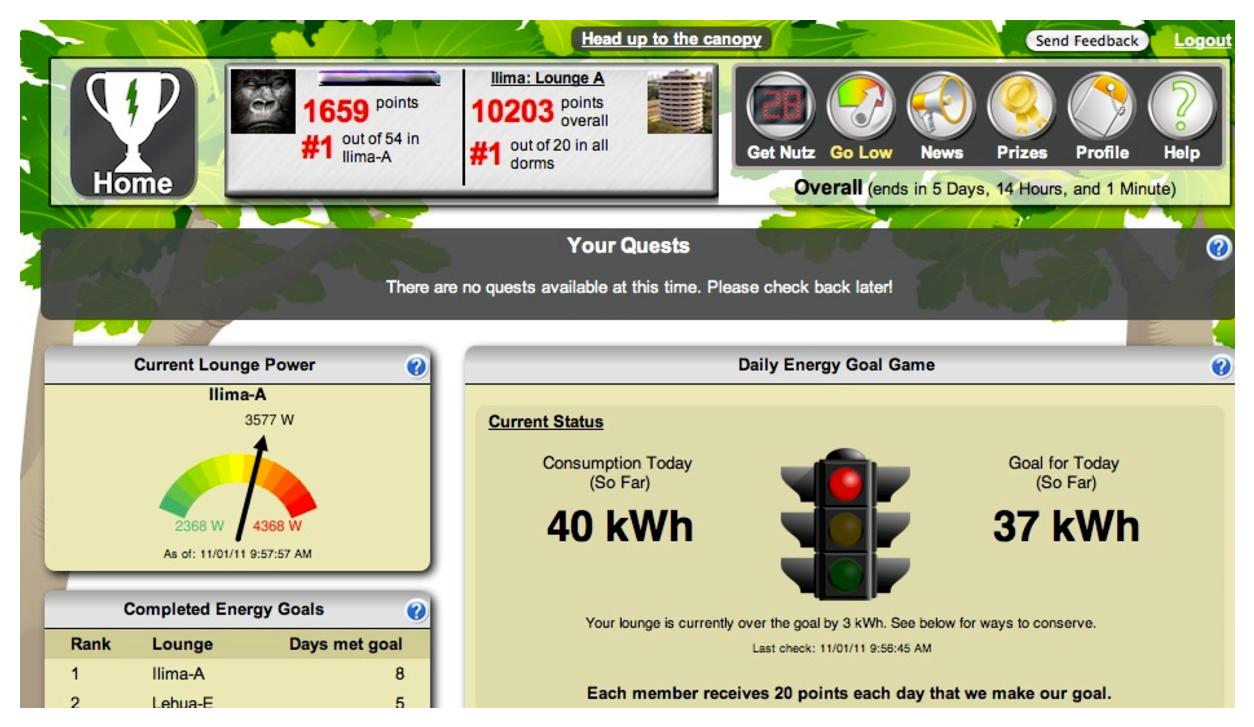
\epsfig{file=golow, width=3in}
\end{center}
\caption{An energy challenge implemented in Makahiki that visualizes WattDepot data}
\label{fig:golow}
\end{figure}

Response to this initial challenge was very positive.   Over 400 students participated, for an adoption rate of approximately 40\%.  In a survey of those participating students conducted near the end of the challenge, over 90\% of them said they would play the game if it were offered next year.  60\% of participants said ``ease of use'' was the thing they liked best about the website.  40\% responded ``Nothing'' when asked what was confusing about the website, and 32\% responded ``Nothing'' when asked what they would change about the website.  The survey did yield insights into what could be improved, including the ability to introduce new games at points during the challenge, to provide better access to other player data, and simplify navigation.

The full version of this paper will go into more detail on our experiences as well as the changes and enhancements we have made to the Makahiki+WattDepot software stack in preparation for three energy challenges by different organizations to be held in Fall, 2012.
